
%%%%%%%%%%%%%%%%%%%%%%%%%%%%%%%%%%%%%%%%%%%%%%%%%%%%%%%%%%%%%%%%%%%%%%%%%
%       Capítulo 2: Descripción de un robot de 5 grados de libertad     %
%%%%%%%%%%%%%%%%%%%%%%%%%%%%%%%%%%%%%%%%%%%%%%%%%%%%%%%%%%%%%%%%%%%%%%%%%

\chapter{\textcolor{Azul}{Descripción de un robot de 5 grados de libertad}}

\section{Articulaciones y pares cinemáticos}

La movilidad de un sistema puede expresarse en función de los parámetros independientes mínimos que se necesitan para describir de manera única su posición y orientación en un instante de tiempo (Norton, 2009). Estos parámetros reciben por nombre \textbf{grados de libertad} (GDL). El número de GDL también depende de las dimensiones del espacio en el que se trabaje. Para ejemplificar el caso del movimiento en un espacio plano de dos dimensiones se puede tomar un cuadrado de papel y colocarlo sobre un escritorio, el papel puede moverse de manera vertical (primer GDL), horizontal (segundo GDL) o girar (tercer GDL). Dichos movimientos también pueden limitarse. Si ahora se toma un alfiler y se clava el cuadrado de papel sobre el escritorio se han restringido los movimientos horizontales y verticales, quedando únicamente la rotación alrededor del alfiler (solamente un GDL).\\\\En el caso del movimiento plano, los cuerpos rígidos sin restricción cuentan con tres GDL, dos que indican posición y uno que indica orientación. Si se considera ahora el espacio tridimensional, los cuerpos rígidos cuentan con seis GDL, se necesitan tres para definir la posición y otros tres que definen la orientación. \\

\\Los eslabones que componen a un robot manipulador están conectados de tal manera que se permita cierto tipo de movimiento. Existen dos movimientos a partir de los cuales se derivan cualquier movimiento complejo conocido: la traslación pura y la rotación pura. Estas conexiones entre eslabones reciben el nombre de articulaciones o pares cinemáticos, Fig (\ref{pares})

\begin{figure}
	\centering
	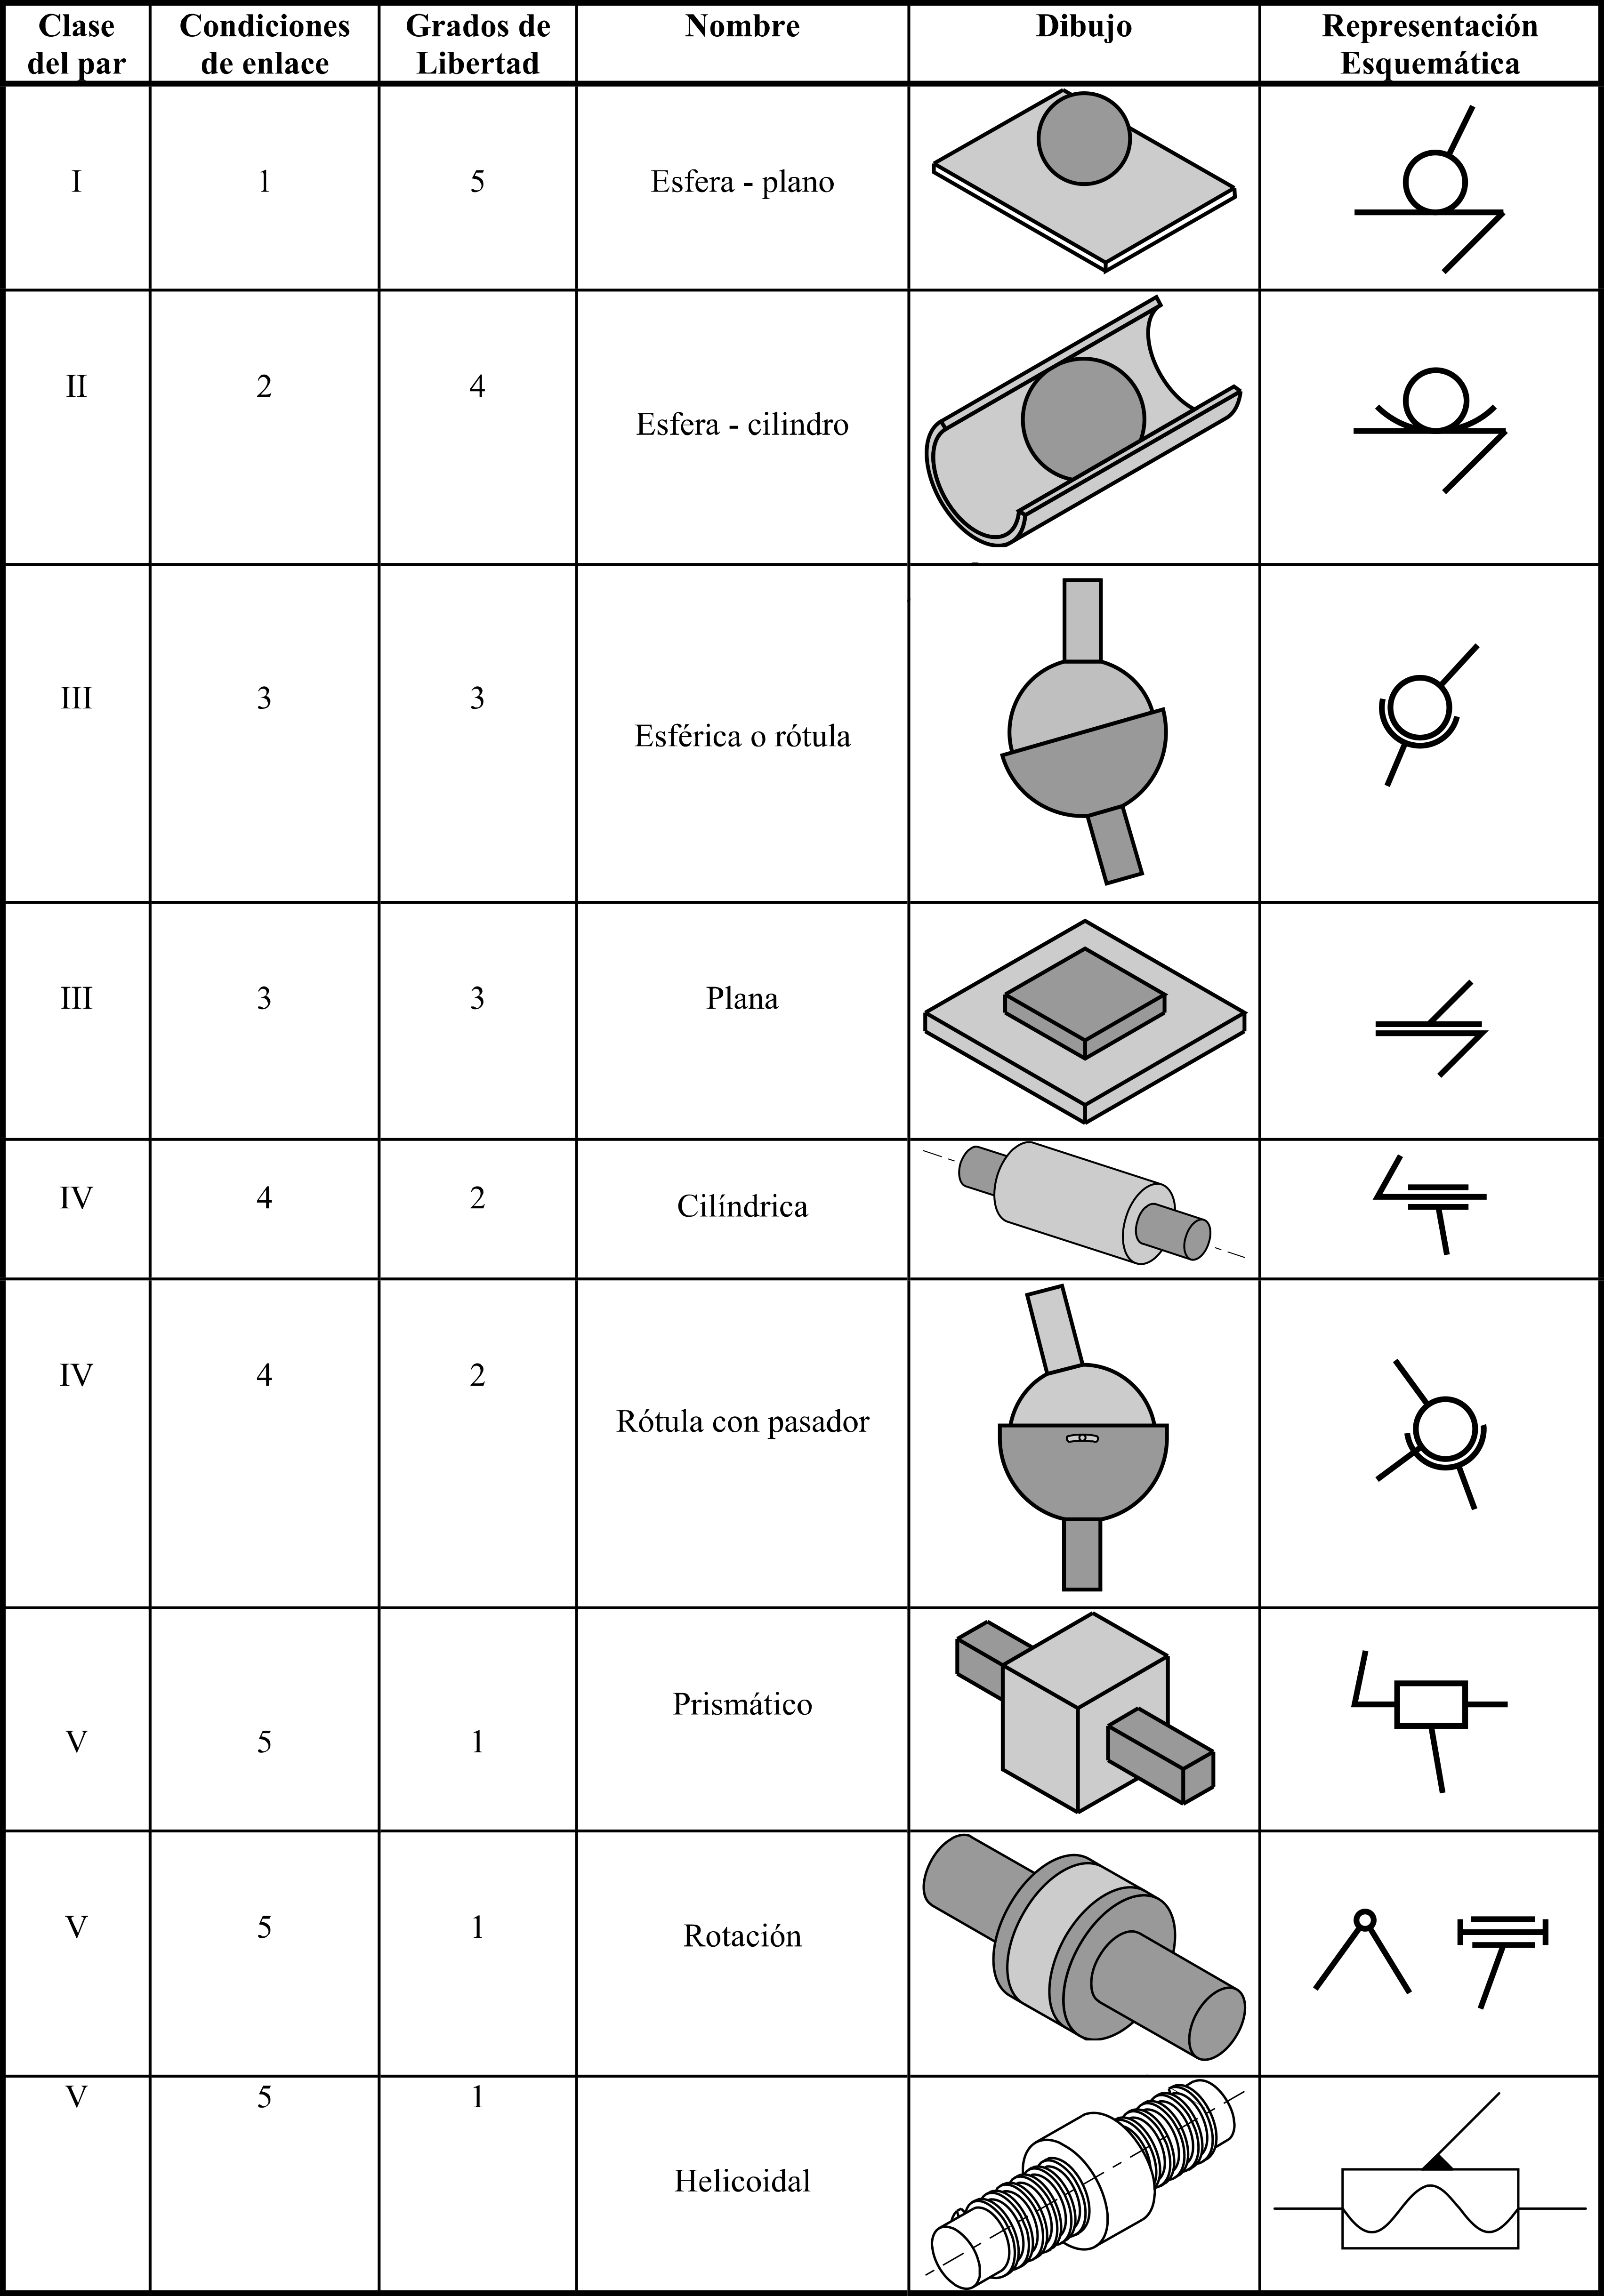
\includegraphics[scale=1.0]{Capitulo2/figs/pares.png} 
	\caption{Pares cinemáticos superiores e inferiores}
	\label{pares}
\end{figure}

\section{Cinemática directa}

Los robots rígidos guardan una relación entre la posición individual de cada articulación y la ubicación espacial de la herramienta o efector final. El propósito de la cinemática directa es determinar los valores de posición y orientación del efector final dados los valores de cada articulación en el robot. 

\subsection{Posición}

\subsection{Orientación}

\section{Cinemática inversa}

\section{Modelado}

%inserción de codigo de Matlab
%Es conveniente sangrarlo (los de proteco dicen "indentarlo") para que no se encime con los números de las líneas a la izquierda
\begin{lstlisting}[frame=single]
    % Declaracion de las variables simbolicas
\end{lstlisting}